\documentclass{article}

\usepackage{graphicx}
\usepackage{tikz}
\usepackage{tikzsymbols}
\usetikzlibrary{calc,patterns,shapes.geometric}
\pagestyle{empty}
\usepackage[margin=0pt]{geometry}
\geometry{papersize={14in,12in}}

\def\centerarc[#1](#2)(#3:#4:#5){\draw[#1] ($(#2)+({#5*cos(#3)},{#5*sin(#3)})$) arc (#3:#4:#5);}

\begin{document}
	\begin{figure}
		\centering
		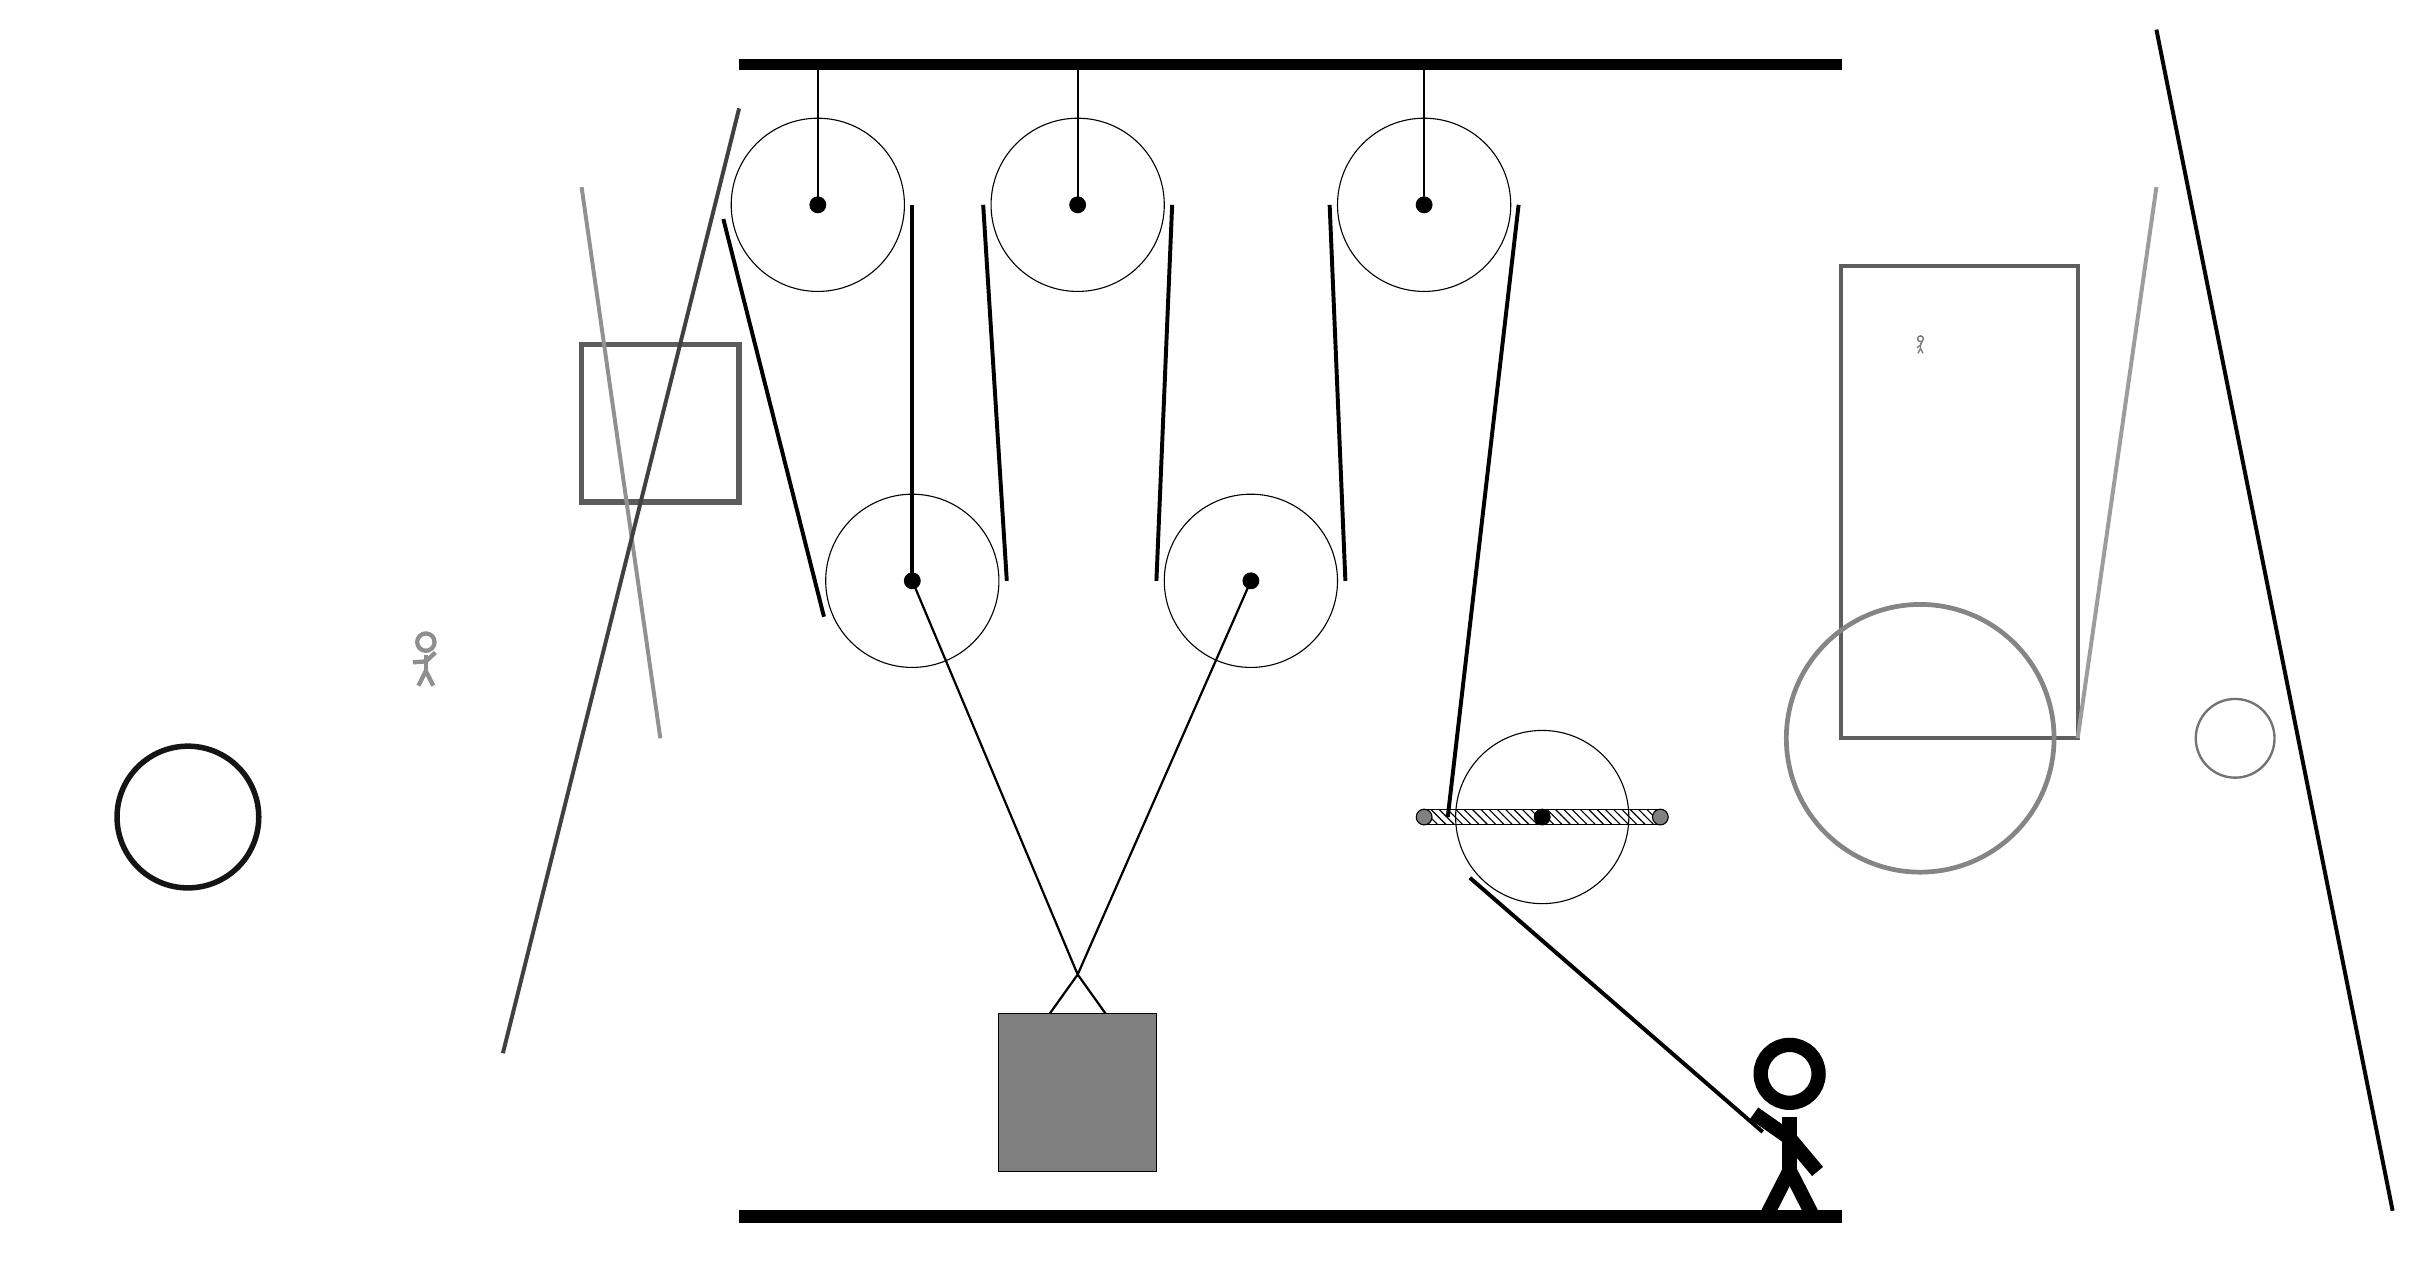
\begin{tikzpicture}
			%%%%% START %%%%%
			
			\draw[fill=black] (-2, 11.5) rectangle (12, 11.625);
			
			\draw (-1, 9.775) circle (1.1);
			\draw[fill=black] (-1, 9.775) circle (0.1);
			\draw[thick] (-1, 9.775) -- (-1, 11.5);
			
			\draw[line width=0.7mm, color=black!64] (-4, 8) rectangle (-2, 6);
			
			\draw [line width=0.7mm, color=black!51](-11, 7) circle (0.0);
			\draw[line width=0.5mm, color=black!63] (12, 9) rectangle (15, 3);
			\draw [line width=0.3mm, color=black!55](17, 3) circle (0.5);
			\node[line width=0.6mm, color=black!44] at (-6, 4) {\Strichmaxerl[3][4][43]};
			
			\draw [line width=0.6mm, color=black!48](13, 3) circle (1.7);
			\node[line width=0.7mm, color=black!52] at (13, 8) {\Strichmaxerl[1][36][67]};
			
			\draw[line width=0.5mm, color=black!98](16, 12) -- (19, -3);
			\draw [line width=0.7mm, color=black!92](-9, 2) circle (0.9);
			
			\draw[line width=0.5mm, color=black!43](-4, 10) -- (-3, 3);
			\draw[line width=0.5mm, color=black!75](-5, -1) -- (-2, 11);
			\draw[line width=0.5mm, color=black!39](16, 10) -- (15, 3);
			
			\draw (2.3, 9.775) circle (1.1);
			\draw[fill=black] (2.3, 9.775) circle (0.1);
			\draw[thick] (2.3, 9.775) -- (2.3, 11.5);
			
			\draw (6.7, 9.775) circle (1.1);
			\draw[fill=black] (6.7, 9.775) circle (0.1);
			\draw[thick] (6.7, 9.775) -- (6.7, 11.5);
			
			\draw (0.2, 5) circle (1.1);
			\draw[fill=black] (0.2, 5) circle (0.1);
			
			\draw (4.5, 5) circle (1.1);
			\draw[fill=black] (4.5, 5) circle (0.1);
			
			\draw (8.2, 2.0) circle (1.1);
			\draw[fill=black] (8.2, 2.0) circle (0.1);
			\draw[pattern=north west lines, pattern color=black] (6.7, 2.1) rectangle (9.7, 1.9);
			\draw[fill=black!50] (6.7, 2.0) circle (0.1);
			\draw[fill=black!50] (9.7, 2.0) circle (0.1);
			
			\draw[thick] (0.2, 5) -- (2.3, 0)  -- (4.5, 5);
			\draw[thick]  (1.8, -0.7) -- (2.3, 0) -- (2.8, -0.7);
			\draw[fill=black!50] (1.3, -0.5) rectangle (3.3, -2.5);
			
			\draw[line width=0.5mm] (0.2, 5) -- (0.2, 9.775);
			\centerarc[line width=0.5mm](-1, 9.775)(0:200:1.2000000000000002);
			\draw[line width=0.5mm] (-2.2, 9.595) -- (-0.922, 4.544);
			\centerarc[line width=0.5mm](0.2, 5)(200:360:1.2000000000000002);
			\draw[line width=0.5mm](1.4, 5) -- (1.1, 9.775);
			\centerarc[line width=0.5mm](2.3, 9.775)(0:180:1.2000000000000002);
			\draw[line width=0.5mm] (3.5, 9.775) -- (3.3, 5);
			\centerarc[line width=0.5mm](4.5, 5)(180:360:1.2000000000000002);
			\draw[line width=0.5mm] (5.7, 5) -- (5.5, 9.775);
			\centerarc[line width=0.5mm](6.7, 9.775)(0:180:1.2000000000000002);
			\draw[line width=0.5mm](7.9, 9.775) --  (7.0, 2.0);
			\centerarc[line width=0.5mm](8.2, 2.0)(180:220:1.2000000000000002);
			\draw[line width=0.5mm](7.2808, 1.2286) -- (11, -2);
			
			\node at (11.3, -2) {\Strichmaxerl[10][-35][-50]};
			
			\draw[fill=black] (-2, -3) rectangle (12, -3.15);
			
			%%%%% END %%%%%
		\end{tikzpicture}
	\end{figure}	
\end{document}